\documentclass[a4paper,14pt]{article}
\usepackage{float}
\usepackage{extsizes}
\usepackage{amsmath}
\usepackage{amssymb}
\everymath{\displaystyle}
\usepackage{geometry}
\usepackage{fancyhdr}
\usepackage{multicol}
\usepackage{graphicx}
\usepackage[brazil]{babel}
\usepackage[shortlabels]{enumitem}
\usepackage{cancel}
\usepackage{textcomp}
\columnsep=2cm
\hoffset=0cm
\textwidth=8cm
\setlength{\columnseprule}{.1pt}
\setlength{\columnsep}{2cm}
\renewcommand{\headrulewidth}{0pt}
\geometry{top=1in, bottom=1in, left=0.7in, right=0.5in}

\pagestyle{fancy}
\fancyhf{}
\fancyfoot[C]{\thepage}

\begin{document}
	
	\noindent\textbf{6FMA50 - Matemática} 
	
	\begin{center}Laboratório de construção de sólidos geométricos (Versão estudante)
	\end{center}
	
	\noindent\textbf{Nome:} \underline{\hspace{10cm}}
	\noindent\textbf{Data:} \underline{\hspace{4cm}}
	
	%\section*{Questões de Matemática}
	
	
    \begin{multicols}{2}
    	\noindent \textbf{Atividade 1}\\
    	\textbf{Planificação de um cubo}\\
    	Experiência: você vai pendurar um cubo e estudar a sombra projetada por ele na parede. Gire o cubo para perceber as variações da forma.
    	\begin{itemize}
    		\item Construa, em uma folha de papel à parte, um cubo de acordo com a planificação abaixo. \\
    		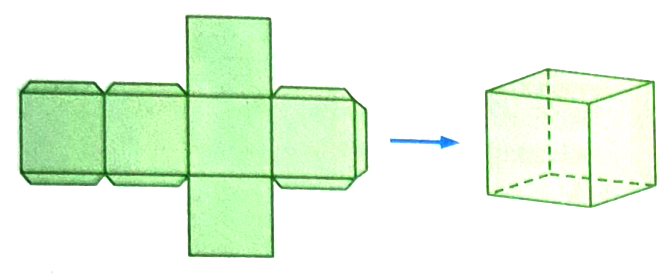
\includegraphics[width=1\linewidth]{imagens_6FMA50/imagem1}
    		\item Com uma fita adesiva, cole um pedaço de linha no centro de uma das faces e ilumine o cubo, analisando suas sombras. Faça o mesmo com a linha em um dos vértices.    		
    	\end{itemize}
        \textbf{Perguntas:}
    	\begin{enumerate}
    		\item Quais são as formas das sombras quando o cubo é pendurado pelo centro da face? \\\\\\\\\\\\\\\\
    	\end{enumerate}
        \noindent \textbf{Atividade 2}\\
        \textbf{Planificação de uma pirâmide}\\
        Construa, em uma folha de papel à parte, uma pirâmide de acordo com a planificação abaixo. \\\\
        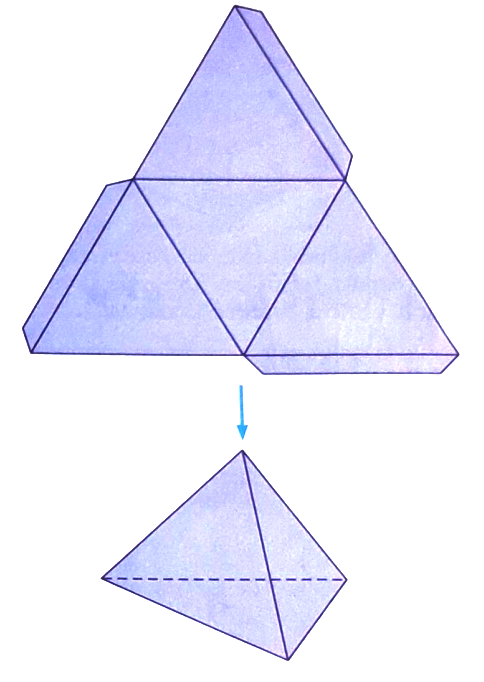
\includegraphics[width=1\linewidth]{imagens_6FMA50/imagem2}
        \textbf{Perguntas:}
        \begin{enumerate}
        	\item Quantos vértices, quantas faces e quantas arestas tem a pirâmide construída? \\\\\\\\\\\\
        	\item As pirâmides cujas faces são todas triangulares têm um nome especial. Qual é? \\\\\\\\\\\\\\\\\\\\\\\\\\\\\\\\\\\\\\
        	\item As faces são triângulos de lados iguais. Como se chamam triângulos cujos lados têm a mesma medida? \\\\\\\\\\\\\\\\\\\\\\\\\\\\
        	\item Procure uma maneira de medir ou estimar a altura da pirâmide que você construiu. Compare o seu resultado com os de outros colegas. \\\\\\\\\\\\\\\\\\
        \end{enumerate}
    \textbf{Desafio olímpico}\\
    (OBMEP) Em um dado a soma dos números de duas faces opostas é sempre 7. Dois dados iguais foram colocados como na figura. Qual é a soma dos números que estão nas faces coladas?
    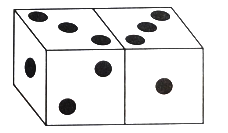
\includegraphics[width=1\linewidth]{imagens_6FMA50/imagem3}
    
    \begin{enumerate}[a)]
    	\item 8
    	\item 9
    	\item 10
    	\item 11
    	\item 12
    \end{enumerate}
    $~$ \\ $~$ \\ $~$
    \end{multicols}
\end{document}